%%%%%%%%%%%%%%%%%%%%%%%%%%%%%
% SCRATCH2: NOT TOOL-SPECIFIC
%%%%%%%%%%%%%%%%%%%%%%%%%%%%%%%%%%%%%%%%%%%%%%%%
%%%%%%%%%%%%%%%%%%%%%%%%%%%%%%%%%%%%%%%%%%%%%%%%
\newpage
\section{SCRATCH2: PARTS OF PIM}
\label{exp-study:qual-results}
%%%%%%%%%%%%%%%%%%%%%%%%%%%%%%%%%%%%%%%%%%%%%%%%
%%%%%%%%%%%%%%%%%%%%%%%%%%%%%%%%%%%%%%%%%%%%%%%%
% This section reports findings from the analysis of the interview notes: comments from the participant annotated with the researcher's observations. The section is structured as follows.


\newpage
%%%%%%%%%%%%%%%%%%%%%%%%%%%%%%%%%%%%%%%%%%%%%%%%
\subsection{Comparing the characteristics of the three collections}
\label{exp-study:item_characteristics}
%%%%%%%%%%%%%%%%%%%%%%%%%%%%%%%%%%%%%%%%%%%%%%%%

This section summarises the general characteristics of the collections of document files, email and web bookmarks. 
Characteristics are presented in terms of:
(1) the nature of the items stored in each collection,
(2) the nature of each collection as a whole,
(3) the nature of the tools used to manage each collection,
and (4) the existence of other collections containing the same type of information.
These characteristics are referred to later in the chapter as factors contributing to the choice of particular PIM strategies (\textit{CHECK}).


\subsubsection{Characteristics of the items stored in each collection}
%%%%%%%%%%%%%%%%%%%%%%%%%%%%%%%%%%%%%%%%%%%%%%%%%%%%%%%%%%%%%%%%%%%%%%

\textbf{Table~\ref{table:chapter3_item_characteristics}} compares the key characteristics of document files, email messages and web bookmarks. 
Emails are clearly differentiated in terms of \textit{authorship} -- the majority of email messages are authored by users other than the owner of the email collection.
For this reason there is a need for users to ascertain the value of email messages after they have been acquired (see \textbf{Section~\ref{exp-study:qual_acquisition}}).
In contrast document files and web bookmarks are explicitly created by the owner of the collection.  
A second key difference is in terms of item \textit{form}.
Email messages and the vast majority of document files contain locally-stored content, much of which has been authored or edited by the managing user.
However web bookmarks are references to content stored remotely on websites
\footnote{Document file collections also facilitate the creation of references that point to other files. These are known as \textit{short-cuts} under MS Windows or \textit{links} under UNIX. However in this study only one user mentioned the regular use of document links (in their case a link to a network drive from their UNIX home directory). Document links were observed more frequently for managing applications on the desktop.}.

\begin{table}[h]
\begin{center}
\begin{footnotesize}
\begin{tabular}{|p{2.5cm}|p{3.5cm}|p{3.5cm}|p{3.5cm}|}
\hline
 & {\bf Document File} & {\bf Email} & {\bf Web Bookmark} \\
\hline \hline
{\bf Creation of items} & Created by owner & Created when messages are downloaded & Created by owner \\
\hline
{\bf Form of items} & Most contain content (e.g. text).  Some references (known as links or short-cuts)  to other  files may also be  present & Contain content (electronic correspondence).  & References to remote web pages on the internet \\
\hline
{\bf Authorship of item content} & Many files are authored/edited by owner of collection.  Some are authored by other users (e.g. downloads).  & Majority of emails authored by other users. Some may be self-addressed or copies of sent messages & Bookmarks do not contain content \\
\hline
{\bf Compound-nature of items} & Files may contain embedded bookmarks, or even other files (e.g. zip archives) & Emails may contain "attached" files or bookmarks & Non-compound \\
\hline
{\bf Homogeneity of items} & Many different types of document file format (e.g. reports, source code, images) & Homogenous & Homogenous \\
\hline
{\bf Life expectancy of items} & Varies but many are kept over the long-term (e.g. over job changes) & Varies but relatively more ephemeral then document files & Tend to be emphemeral, users forget about them and webpages are themselves volatile. Can be considered as short-term ``expressions of interest'' \\
\hline
\end{tabular}  
\end{footnotesize}
\caption{Comparing the characteristics of file, email and bookmark items}
\label{table:chapter3_item_characteristics}
\end{center}
\end{table}
\normalsize




\newpage
\subsubsection{Nature of each collection}
%%%%%%%%%%%%%%%%%%%%%%%%%%%%%%%%%%%%%%%%%

\textbf{Table~\ref{table:chapter3_collection_characteristics}} presents a summary of the underlying characteristics of each collection.  Documents and email were collected much more extensively than bookmarks.  Document file collections were the most highly valued, and often contained items that had been kept over many years (Subject 13: \textit{``my environment has evolved over 12 years''}).  Email collections were seen as being relatively less valuable than document files, although many users mentioned the presence of important messages of a work-related or sentimental nature.  In contrast, bookmark collections were of little importance to their owners, and many used alternate mechanisms for finding websites such as search engines even if they had recorded the relevant bookmark previously.
% A number of users did not collect bookmarks at all (COUNT, COMPARE WITH DOCS AND EMAIL), and many tended to u (CHANGE).
\begin{quote}
Subject 1: \textit{``Its often not worth the overhead of adding links, I only use the pages once or twice. And then there's the overhead of managing the organization.''}
\end{quote}

\begin{table}[h]
\begin{center}
\begin{footnotesize}
\begin{tabular}{|p{2.5cm}|p{3.5cm}|p{3.5cm}|p{3.5cm}|}
\hline
	& {\bf Document File} & {\bf Email} &  {\bf Web} \\
\hline \hline
{\bf Size of collection} & Large (many hundreds) & Very large (thousands) & Small (tens) \\
\hline
{\bf Importance of collection} & Very important. Often taken with user when they change job. & Somewhat important (especially recent items in inbox).  & Management typically not seen as a priority by users. Bookmark collections often abandoned (COUNT) \\
\hline
{\bf Age of collection} & Many years.  & A few years. & Less than a year.   \\
\hline
{\bf Context of collection} & Distinct by default, but separation not enforced so personal files often co-exist with system files & Distinct collection contained within mail reader-specific store. & Distinct collection typically contained within web browser-specific store. \\
\hline
{\bf Currency of collection} & Substantial minority of active files relating to current projects and interests. Majority are effectively archived but are held in some value & A substantial number of the messages in inbox are typically active.  Overall majority of items are effectively archived and not in use & Small minority active - typically those added most recently \\
\hline
\end{tabular}  
\end{footnotesize}
\caption{Comparing the characteristics of the document file, email and web  collections}
\label{table:chapter3_collection_characteristics}
\end{center}
\end{table}
\normalsize


\newpage
\subsubsection{Existence of other collections of each type of information}
%%%%%%%%%%%%%%%%%%%%%%%%%%%%%%%%%%%%%%%%%%%%%%%%%%%%%%%%%%%%%%%%%%%%%%%%%%

Numerous cases were observed when the management of a particular type of information was distributed across multiple distinct collections.
For instance many users managed document files using several parallel mechanisms within their primary digital workspace: (1) within the file system, (2) spatially as desktop icons, and (3) as email attachments. 
This distribution of the management of a particular type of information has been referred to as \textit{compartmentalization}~\cite{Bellotti:00}. \textbf{Table~\ref{table:chapter3_other_collections}} summarizes our observations of the compartmentalization of document files, email, and web bookmarks -- both within the primary digital workspace, and across the extended personal workspace\footnote{Compartmentalization was also observed for other types of personal information such as contacts and to-do items.  For instance contacts were fequently scattered between email, personal diaries, notebooks, and mobile phones.}. Issues and problems relating to the compartmentalization of document files, email and web bookmarks is discussed in more detail in \textbf{Section~\ref{exp-study:ct}}



\begin{table}[h]
\begin{center}
\begin{footnotesize}
\begin{tabular}{|p{2.5cm}|p{3.5cm}|p{3.5cm}|p{3.5cm}|}
\hline
	& {\bf Document File} & {\bf Email} &  {\bf Web} \\
\hline \hline
{\bf Inside primary desktop workspace} & Document files can also be managed as desktop icons or as email attachments.  & Emails typically managed only within email tool, although they can also be stored as desktop icons. & Web bookmarks often managed as desktop icons or as embedded links within emails or documents.  \\
\hline
{\bf Outside primary desktop workspace} & Network drives. Personal document files stored on other computers or PDAs. & Email stored on other computers or devices. Web-email collections (such as Yahoo! Or Hotmail) & Web bookmarks stored on other computers or devices.  \\
\hline
\end{tabular}  
\end{footnotesize}
\caption{Existence of other collections}
\label{table:chapter3_other_collections}
\end{center}
\end{table}
\normalsize
%%%%%%%%%%%%%%%%%%%%%%%%%%%%%%%%%%%%%%%%%%%%%%%%

% \noindent
\subsubsection*{NOTES ON SECTION~\ref{exp-study:item_characteristics}}
%%%%%%%%%%%%%%%%%%%%%%%%%%%%%%%%%%%%%%%%%%%%%%%%%%%%
\begin{footnotesize}
\begin{itemize}
	\item \textit{Point out that these are average figures. Meant to be typical/average}
	\item \textit{NOTE: no objective figures regarding size of collections}
	\item \textit{QUANT: mention numbers for qualitative observations}
	\item \textit{FIGURE: label features in abstract representation}
	\item \textit{MOVE: move pim-tool abstraction to chapter 2}
\end{itemize}
\end{footnotesize}





\newpage
%%%%%%%%%%%%%%%%%%%%%%%%%%%%%%%%%%%%%%%%%%%%%
\subsection{Comparing Acquisition Strategies}
\label{exp-study:qual_acquisition}
%%%%%%%%%%%%%%%%%%%%%%%%%%%%%%%%%%%%%%%%%%%%%

Barreau defined acquisition as the methods and rules by which information becomes part of the PIM system~\cite{barreau:95}.
\textbf{Table~\ref{table:chapter3_acquisition_strategy}} compares the main characteristics of acquisition behaviour between the PIM tools.
In our study we noted substantial differences regarding the acquisition of document files and web bookmarks on one hand, and email on the other.
The acquisition of document files and web bookmarks is under the user's explicit control. Items are added to the collection manually as driven by their needs and interests.
In contrast email acquisition is effectively uncontrolled. 
Any items sent to the user concerned appears in their collection be it important work mail or distracting spam.
As Subject 11 put it: \textit{``everything just gets stuffed into the inbox -- basically the whole world has write access!''}. 
The user has little control over what items are added beyond specifying when new messages are downloaded, the use of mail filters to delete spam and the act of unsubscribing from mailing lists that are no longer of interest. 
This points to two very different modes of acquisition.
In the document file and web bookmark colections, the user decides what items to add. 
In email the onus is on the user to assess the value of items and decide what to delete.  For some users the presence of unwanted messages was not a problem. Others complained about the significant amount of effort involved in processing new email:

\begin{quote}
	Subject 21 (EMAIL): \textit{``I try to keep it [the inbox] as small as possible, so it acts as a to-do list. I have another folder called `Diverse' which is stuff to deal with thats been tidied from inbox''}
\end{quote}

\begin{table}[h]
\begin{center}
\begin{footnotesize}
\begin{tabular}{|p{2.5cm}|p{3.5cm}|p{3.5cm}|p{3.5cm}|}
\hline
    {\bf } & {\bf Document File} & {\bf Email} & {\bf Web Bookmark} \\
\hline \hline
{\bf Item acquisition} & Manual creation. Explicitly saved by user (whether items are authored or downloaded) & Automatic creation. Items created when downloaded from mail server.  & Manual creation. \\
\hline
{\bf Creation rate of items} & Low  (estimate: 1-5 per day on average) & High (many users receive dozens every day) & Low (estimate: 1-2 per day on average) \\
\hline
{\bf Main user activity} & Deciding what to add (low overhead) & Ongoing management of inbox --processing new mail (high overhead).  & Deciding what to add (low overhead) \\
\hline
{\bf Need for assessment of value} & Users typically only create items of some perceived value & Yes. Large overhead in evaluating items and deciding what to keep/deal with/delete & Users typically only create items of some perceived value \\
\hline
{\bf Likelihood of keeping acquired items} & High.  Acquired items are rarely deleted. & Low. Many items acquired are deleted. & High. Most created bookmarks are not subsequently deleted (however many users had abandoned entire collection and started over) \\
\hline
{\bf Naming of items} & Each item must have a unique name. & Default "name" is defined by Subject line as specified by sender. Typically hard to change & Default named is title of the page to which bookmark refers. \\
\hline
{\bf Standard implicit metadata assigned by system} & Date-created, date-modified, size, author & Date-received, from, to, threading information, size & Date-created, date-modified, size author \\
\hline
\end{tabular}  
\end{footnotesize}
\caption{Comparing Acquisition Practices between the Tools}
\label{table:chapter3_acquisition_strategy}
\end{center}
\end{table}




\newpage
%%%%%%%%%%%%%%%%%%%%%%%%%%%%%%%%%%%%%%%%%%%%%%
\subsection{Comparing Organization Strategies}
\label{exp-study:qual_organization}
%%%%%%%%%%%%%%%%%%%%%%%%%%%%%%%%%%%%%%%%%%%%%%

In the conceptual overview of PIM presented in \textbf{Section~\ref{ch1:research-area}} we considered two forms of organization within PIM systems: (1) implicit organization based on system-assigned metadata, (2) explicit organization performed by the user (e.g. classifying items within folders or spatially grouping items on the desktop). 
In this study we focused on the users' explicit organizing behaviour exhibited by the study participants in their document file, email and web bookmark collections.
\textbf{Table~\ref{table:chapter3_organization_strategy}} provides an overview of our findings.
\\

\noindent
By far the dominant explicit organizational mechanism employed was the folder hierarchy. Desktop icons were used by about half the users (specify)to manage document files or web bookmarks on a temporary ``work in progress'' basis. 
Note that other collections of personal information such as contacts and to-do items were rarely organized explicitly.
Although organizing behaviour varied between users, common approaches stood out for each type of information. \textbf{Figure~\ref{fig:chapter1_collection_forms}} illustrates the typical forms of the document file, email and web bookmark collections that we encountered. 
Overall the document file collection tended to be structured much more extensively with the vast majority of items filed within folders for most users.
On average the file folder hierarchies were almost twice as deep as the email and web bookmark hierarchies (see \textbf{Table~\ref{table:chapter3_organization_strategy}}). 

% %%%%%%%%%%%%%%%%%%%%%%%%%%%%%
% FIGURE - FOLDER SHAPES
% %%%%%%%%%%%%%%%%%%%%%%%%%%%%%
\begin{figure}%[t]
	\begin{center}
		\leavevmode
		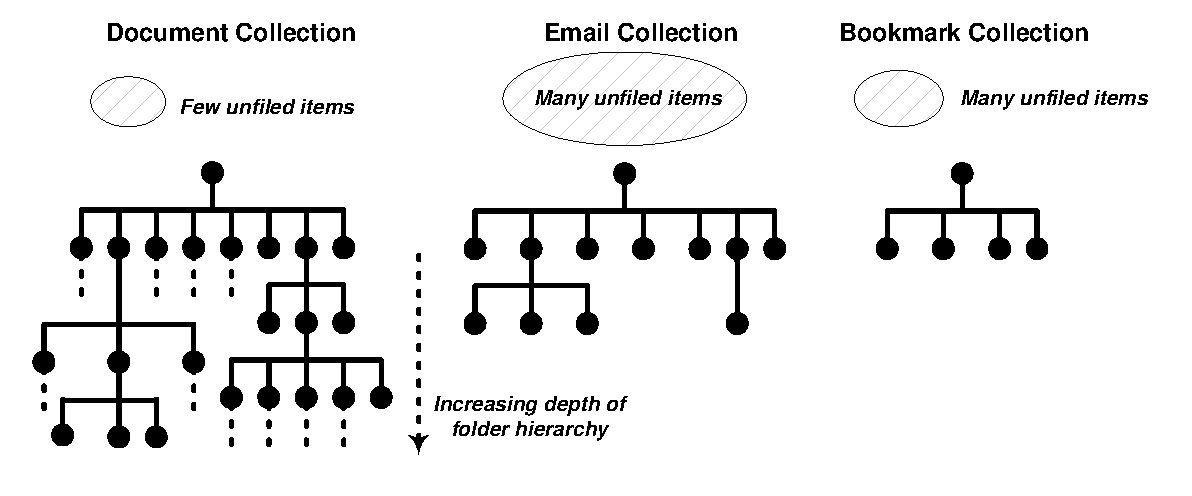
\includegraphics[width= \textwidth]{pictures/exp-study/exp-study-OrgComparison.pdf}
		\caption{Comparison of the typical form of folder hierarchies developed in each PIM collection}
		\label{fig:chapter1_collection_forms}
	\end{center}
\end{figure}


% DOCUMENT FILES
\noindent
Twenty-three of the twenty-five participants had document file folders in active use~\footnote{An active folder was defined as one containing items that were used in the last week/on a regular basis.}. Most of these subjects pursued a \textit{file-on-creation} strategy with their document files: as items were created, users habitually filed them away (either using the file manager or the file dialog within editors such as MS Word).
\\

\noindent % EMAIL
Users were generally less reliant on folders in their email collection, and only twenty of the participants had folders that were in active use.  The average number of folders was lower than in the document collection (34.1 compared to 42.6).
During the guided tours of their email collections, users talked about organization in terms of keeping their inbox tidy.
This \textit{inbox-focused} organizing tended to be as much about deleting items as filing them away in folders. 
The most common user strategy was a combination of incremental deletion and filing of messages when they were ``dealt with'' (e.g. read or replied to).  The subjects indicated that their inboxes often got ``out of control'' so the incremental organizing was backed-up with occasional spring-cleans. Several users (\textit{COUNT}) also used filters to automatically delete or file certain messages.  Five subjects did not file email. Instead they relied on implicit metadata-based organization to help them locate items.

\begin{quote}
	Subject 13 (email): \textit{``I try and file systematically but right now my inbox is pretty big because I had no time over Christmas''}
\end{quote}

\noindent
Bookmarks tended to be less structured than the other two collections with most items being left in a chronologically ordered list.  Less than half the users had web bookmark folders in active use. 
Several users indicated that both web bookmarks and email had less value than document files and so were less worth organizing.

\begin{quote}
	Subject 19 (EMAIL): \textit{``I've just happened to start filing as an experiment.  But I worry that its just like filing trash -- like having a tidy waste paper basket.''}
\end{quote}

\begin{quote}
Subject 1 (BOOKMARKS): \textit{``Its often not worth the overhead of adding links, I only use the pages once or twice. And then there's the overhead of managing the organization.''}
\end{quote}

\noindent
During the study we estimated the number of folders in active use based on user comments. An active folder was defined as one containing items that had been filed or retrieved in the last week (\textit{OR: on a regular basis}). Overall more of the document file and email folders tended to be in active use compared to the web bookmark folders.  Although no quantitative measures were taken, many users mentioned that their web bookmark folders were old and/or redundant. An interesting further experiment would be to harvest currency information about the categories used in each classification scheme.
\\

\begin{table}[h]
\begin{center}
\begin{footnotesize}
\begin{tabular}{|p{2.5cm}|p{3.5cm}|p{3.5cm}|p{3.5cm}|}
\hline
    {\bf } & {\bf Document File} & {\bf Email} & {\bf Web Bookmark} \\
\hline \hline
{\bf Number of users with active folders (n=25)} &         23 &         20 &         12 \\
\hline
{\bf Average number of folders (n=25)} &       42.6 &       34.1 &       11.2 \\
\hline
{\bf Average maximum depth of folders (n=25)} &        2.3 &        1.4 &        1.1 \\
\hline
{\bf Most common organizational strategy (filers only) } & "One touch" file-on-creation & Incremental filing (and deleting) after items "dealt with.  Occasional spring-cleaning (filing and deleting). Use of filters for mailing lists.  & Mostly tend to leave in default chronological list. However if users file, they file, file soon after creating.  \\
\hline
{\bf Proportion of items filed (filers only) } & High - approx 95\%. & Medium - approx 40\% (high variability). Large number of unfiled items in "inbox" & Majority in chronologically ordered list \\
\hline
{\bf Proportion of folders in active use (filers only)} & Approx 50\% active & Approx 50\% active & Few folders active. In many cases entire folder hierarchy abandoned \\
\hline
{\bf Key organizational problems (filers only)} & Anxiety of order. Keeping collection tidy (unfiled items, pruning folders).  & Anxiety of order (focused on inbox). Filing/deleting large number of items in inbox & Anxiety of order. Time to organize outweighs value of doing so (items rarely used again). Poor interface for organizing \\
\hline
{\bf Location of "active" items} & Occasional unfiled "work-in-progress" area, but most active files are located in project-specific folders & Inbox. Occasional project folders & Most likely to be recently added items \\
\hline
{\bf Other (non-filing based)  organization methods} & Spatial placement on desktop. Separation of roles on different hard drives and partitions & Separation of roles between accounts and mail readers. & Occasional spatial placement on desktop \\
\hline
\end{tabular}  
\end{footnotesize}
\caption{Comparing Organization Practices between the Tools}
\label{table:chapter3_organization_strategy}
\end{center}
\end{table}


\noindent
Compare results with previous studies (broadly in line):
\begin{itemize}
	\item DOCS: (Barreau and Nardi 1995), EMAIL: Duchaneaut and Bellotti (2001), WEB: ABRAMS ET AL (1998)
	\item Numbers of folders, These results can be compared with those of Duchaneaut and Bellotti (2001) who observed an average of 400 email folders with a median result of 27.
	\item Duchaneaut and Bellotti also observe a correlation between email experience and number of folders. Although this relationship was not rigorously analysed here, several experienced subjects had very few folders - possibly questioning the generality of Duchaneaut and Bellotti's result. \textit{THINK: WHY LOWER HERE ?}
	\item Depth This did not tie in with results from other user studies including (Barreau and Nardi 1995). 
	\item Folder activity (i.e. much of items effectively archived)
\end{itemize}

\noindent
DEVELOP: Other folder-related aspects to discuss:
\begin{itemize}

	\item Consider use of large/small categories, default folders

	\item Mainly store to retrieve. Tendency to file if greater perceived value of information (e.g. important information, if easier to file, or if higher perceived chance of retrieving it again).  Filing tended to be seen as something that aided in retrieval. But there were other uses for folders:
	\begin{itemize}
		\item also consider contextualizing uses of folders (e.g. for reminders, version control etc.)
	\end{itemize}

\end{itemize}

\noindent
DEVELOP: CHOICE OF STRATEGY - KEY FACTORS:
\begin{itemize}
	\item Perceived value of items relative to perceived overheads
	\item Personal disposition towards tidiness -- users either inclined to organize or not
\end{itemize}

\noindent
DEVELOP: USER DISPOSITION TOWARDS FILING
\begin{itemize}
	\item Perceived benefits of being tidy. Mean different to different people. Perceived consequences of organizing
	\item Kirsten quote, worthwhile
	\item Bob quote (more users in email and bookmarks)
\end{itemize}

\begin{quote}
	Subject 11: \textit{``These are ongoing projects which I like to keep tidy as they could be of future importance. Having an organized computer has clear benefits for future research by making it easy to find and read stuff when you need it again.''}
\end{quote}
\begin{quote}
	Subject 6: \textit{``I'd characterise myself as being (1) busy and (2) lazy. I need to carefully priotize my time with a bias towards (1) fun, and (2) must-do/sense of duty.  Since PIM isn't either of these I don't do it!  Basically there's more fun things to do. Somewhere to dump things whilst I do something more interesting''}
\end{quote}

\noindent
DEVELOP: REPORTED PROBLEMS
\begin{itemize}
	\item BIGGEST PROBLEM: Anxiety of order e.g. old/failed/duplicate folders, unfiled items (Subject 21 (DOCS): \textit{``stuff that went there accidently''}). Level of this influenced by user disposition
	\item More space -- more items -- more organizing to do (in the old days people might be more careful about what they acquire and keeping it tidy would therefore be easier)
	\item Paradox - more items, more folders, more organizing to do
	\item Interestingly the other classic technical limitations of the folder hierarchy were rarely mentioned. Classic tree problems (multiple classification, static hierarchy) rarely mentioned (COUNT USERS). Some (failed folders, duplicate folders) mentioned in context of staying tidy
\end{itemize}

\noindent
Evidence of changed strategies. No. Users typically settled in their choice of management strategy	Yes. Several (NUMBER) users had abandoned pro-filing strategies, towards leaving items in inbox. One user  switched  other way.	Yes. Evidence of many users  abandoning pro-filing strategies (NUMBER) or entire collection (NUMBER)

\begin{quote}
	Subject 12 (EMAIL): \textit{``I used to have lots of folders for each sub-project [of a main research area] but there just wasn't enough time to manage them. In an ideal world there'd be a rich structure ... and the hierarchy is now flattened and simplified''}
\end{quote}

\begin{quote}
	Subject 5 (DOCS): \textit{``Now I've got a set of folders and create a new one if I've got too many unfiled.  Historically I use to be less organized and everything was unfiled.  I still have to search for this using type or date metadata.''}
\end{quote}

\noindent
DEVELOP: CLOSE WITH SMALLER GRANULARITY ANALYSIS
\begin{itemize}
	\item Barreau: different classifying rules based upon level of granularity to support in workload
	\item THINK: ADD: Different types of information -- different organizational strategies (e.g. MP3s cf. source code)
	\item MOVING ON Relate to Quant analysis in \textbf{Section~\ref{exp-study:folder-analysis}} and user classification in \textbf{Section~\ref{exp-study:qual_classification}}
\end{itemize}




\noindent
\subsubsection*{NOTES ON SECTION~\ref{exp-study:qual_organization}}
%%%%%%%%%%%%%%%%%%%%%%%%%%%%%%%%%%%%%%%%%%%%%%%%%%%%

\begin{footnotesize}

\begin{itemize}

	\item Carefully differentiate organization (incremental ongoing filing/tidying) and maintenance (occasional spring-cleaning).

	\item ADD/DEVELOP STATS:
	\begin{itemize}
		\item \textit{ADD: median, standard deviations, p-values for comparison?}
		\item \textit{THINK: ADD hierarchy fan-out (interpret as use of small/large categories?)}
		\item Rationalize spring-clean organizing/tidying with maintenance section
	\end{itemize}
	
\end{itemize}

\end{footnotesize}



\newpage
%%%%%%%%%%%%%%%%%%%%%%%%%%%%%%%%%%%%%%%%%%%%%%
\subsection{Comparing Maintenance Strategies}
\label{exp-study:qual_maintenance}
%%%%%%%%%%%%%%%%%%%%%%%%%%%%%%%%%%%%%%%%%%%%%%

\textbf{Table~\ref{table:chapter3_maintenance_strategy}} summarizes our observations from the study regarding maintenance/upkeep/keeping in good condition/good working order/tuning. The following types of maintenance activity were encountered during the study:
\begin{enumerate}
	\item \textbf{item-level tidying} -- at the file-level, at the folder-level, or global ``spring-cleaning'' of the entire collection
	\item \textbf{archiving} -- removing a portion of the collection and placing it in separate storage
	\item \textbf{making back-ups} -- making a copy of the current collection
	\item \textbf{synchronization} -- mirroring the collection between devices
\end{enumerate}

\noindent
Users varied in terms of how much maintenance-related activity was carried out and was strongly dependent on user disposition. 
In terms of tidying, some users were proud of the fact that they had not tidied their files since they had started collecting them! However most users carried out occasional tidying on their collections of personal information.  Tidying was either carried out at the file-level (filing, deleting files), at the folder-level (reorganizing folders), or globally (``spring-cleaning'' the entire collection).
\\

\noindent
Tidying was most commonly referred to in the context of email and was typically focused at deleting and/or filing items in the inbox once it had reached a certain size.  Tidying appeared to be less common in the document file context where items were typically organized incrementally. Tidying was also rare in the context of bookmarks, although for a very different reason.  Bookmark collections were of so little value to users, that many reported their abandonment rather than devoting effort to maintaining them. However interestingly, they would then proceed to start the collection again (EXPAND)
\begin{quote}
	Subject 2 (BOOKMARKS): \textit{``I have lots of unfiled bookmarks as they're hard to file. I could go through and delete them but not high-priority.''}
\end{quote}

\noindent
For those users for whom tidiness was important, spring-cleaning was typically initiated when a collection reached a certain level of messiness. 
Incremental: a) category too big - therefore split into sub-categories, b) category too small (failed folder) -- remove, c)  duplicate folders - merge, d) lose something - improve filing system.
Others were more pragmatic and spring-cleaned when they failed to find an item (e.g. Subject 18: \textit{``If I lose something, then I make the hierarchy richer.''}).
\\

\noindent
The other forms of maintenance were carried out in a satisficing manner as influenced by outside factors (e.g. crash, reinstall, running out of space, new job/life change).
These findings confirmed previous observations: that maintenance is generally dominated by circumstance~\cite{barreau:95}.
Users reported archiving portions of the document file or email collections when they ran out of space\footnote{As computing memory is becoming cheaper there was less evidence of this being an issue than in Barreau's survey~\cite{barreau:95} (NUMBER: ONLY XYZ USERS MENTIONED SPACE BEING AN ISSUE).}, if they were changing computer, or moving to a new job.
\begin{quote}
	Subject 21 (DOCUMENTS): \textit{``there's a lot of stuff that shouldn't have been there ... need to tidy up, I'm always out of memory''}
\end{quote}

\noindent
Most items in the collections were effectively archived in situ, lots of space, no need to archive them. There was some concern at the poor accessibility of archived material.  Again archiving was most common for those users for whom tidiness was important.
\begin{quote}
	Subject 1: ``After the project finished it was 99\% useless stuff. I just wanted to get it out of the way''
\end{quote}

\noindent
Backing-up and synchronization was most commonly observed when it was automatic, for instance the automatic backing-up of a network drive. 
Occasionally highly-important work was explicitly backed up, typically using a ad-hoc manual mechanism.
A number of users expressed the wish for improved synchronization support. Currently carried out in an ad-hoc manner (e.g. by email). Most common for document files. Although users mentioned that they would also like it for email and bookmarks.
\\

\noindent
Maintenance is an activity that users carry out in a satisficing manner~\cite{barreau:95}, typically when forced to by external circumstances.
For instance users only carried out spring-cleans when they were forced to by external factors such as deleting large files when running out of space. 
The end of projects were often mentioned as a time when the user had time to maintain collections and make back-ups.
\\

\noindent
However this meant that certain users had lost data (e.g. jor).
\\

\noindent
Most acknowledge the worth of maintenance but were not willing to devote much time towards it.  Demand for increased provision of automatic support for backing up and synchronrisation. Mostly document files and email.  Not bookmarks.
\\

\begin{table}[h]
\begin{center}
\begin{footnotesize}
\begin{tabular}{|p{2.5cm}|p{3.5cm}|p{3.5cm}|p{3.5cm}|}
\hline
& {\bf Document File} & {\bf Email} & {\bf Web Bookmark} \\
\hline \hline
{\bf Tidying items} & Occasional tidying of unfiled items or reorganization of folders & Occasional tidying of inbox & Very rare. Most likely to abandon entire collection \\
\hline
{\bf Backing-up Practice} & Occasional manual backing-up for important files. Some usage of network drive that are automatically backed up & Rare, although occasionally a copy of all messages left on server & Not reported \\
\hline
{\bf Archiving Practice} & Rarely performed Much of collection is effectively old and "archived" in situ & Rare. Occasionally entire email inbox/collection of non-filers is archived en-masse and started over. Email tools often have built in automatic archiving, e.g. to remove items older than a certain date & Not reported \\
\hline
{\bf Synchronization Practice} & Occasionally performed manually (e.g. from work desktop to laptop) & Occasionally downloaded in parallel on multiple machines. I so, user tends to organize one collection & Not reported \\
\hline
\end{tabular}  
\end{footnotesize}
\caption{Comparing Maintenance Practices between the Tools}
\label{table:chapter3_maintenance_strategy}
\end{center}
\end{table}



\noindent
\subsubsection*{NOTES ON SECTION~\ref{exp-study:qual_maintenance}}
%%%%%%%%%%%%%%%%%%%%%%%%%%%%%%%%%%%%%%%%%%%%%%%%%%%%
\begin{itemize}
\item blah
\end{itemize}






\newpage
%%%%%%%%%%%%%%%%%%%%%%%%%%%%%%%%%%%%%%%%%%%%%%
\subsection{Comparing Retrieval Strategies}
\label{exp-study:qual_retrieval}
%%%%%%%%%%%%%%%%%%%%%%%%%%%%%%%%%%%%%%%%%%%%%%

Unlike acquisition and organization where we observed a wide range of user strategies, approaches to retrieval were more consistent.
Subjects indicated that they only used the integrated search mechanisms present in document file and email managers as a last resort. 
Rather than searching items by metadata or content, users expressed a strong preference for browsing which was seen as the faster alternative. 
The preference for browsing over search confirms results from previous studies of particular tools (e.g.~\cite{bn:95}).
For document files, users expressed a preference for browsing through folders, supported by the sorting of items based on implicit metadata. Additionally many users employed application-history when working in tools such as MS-Word -- thus avoiding the need to browse or search.
In email, retrieval was typically carried out in the inbox by browsing a sorted lists of items.

\begin{quote}
Subject 2 (DOCUMENTS): \textit{`` If I'm looking for something, I'll firstly browse about.  I only search as a last resort. If its something I've downloaded, often its easier just to go to google and download again from the web!''}
\end{quote}

\begin{quote}
Subject 2 (EMAIL): \textit{``I try to minimise structure as I find by sorting on date and sender metadata to get a flexible view.  Then I search if I can't find it.''}
\end{quote}

\begin{quote}
Subject 21 (EMAIL): \textit{``When I'm findings things [messages] first I'll browse for a minute or so. If that doesn't work then I'll search, but thats so slow.''}
\end{quote}

\noindent 
None of the bookmark interfaces encountered provided a search mechanism, and in fact most users indicated that they did not often retrieve the bookmarks they stored. If bookmarks were retrieved they were typically those added most recently or one or two frequently-used links. Instead users were more likely to use an alternate mechanism for accessing web pages such as a search engine.  Despite the lack of preference for search in document files and email, interestingly several participants complained about the lack of a search facility in their bookmark tool.
\\

\noindent 
\textbf{Table~\ref{table:chapter3_retrieval_strategy}} summarizes our observations and analysis. Interestingly findings items did not appear to be as much of a problem as the issue of ``anxiety of order'' reported in \textbf{Section~\ref{exp-study:qual_organization}}.  Users reported that they were able to find items when they needed them on most occasions. However those times when they failed to locate items were quite rare, they were very frustrating. Several users reported looking for items for about ten minutes before resorting to an alternative method (e.g. asking a correspondent to resend an email). Several users reported that the compartmentalization of documents across tools lead to problem sof retrieval, especially in the case that they were looking for a particular copy of a document between the file system and email attachments.
\begin{quote}
	\textit{INSERT Subject 22's comment of not being able to find item of email and the consequence of that!}
\end{quote}

\begin{table}[h]
\begin{center}
\begin{footnotesize}
\begin{tabular}{|p{2.5cm}|p{3.5cm}|p{3.5cm}|p{3.5cm}|}
\hline
    {\bf } & {\bf Document File} & {\bf Email} & {\bf Web Bookmark} \\
\hline \hline
{\bf Likelihood of access/retrieval} & High for work in progress. Occasional for archived items. & High for recent items in inbox. Low for archived. & Low. Bias towards items recently added. \\
\hline
{\bf Dedicated search mechanism} &        Yes &        Yes &         No \\
\hline
{\bf Preferred retrieval strategy} & Browse (supported by sort). Search as last resort. & Sorting of inbox, sorting combined with browsing into folders. Search as last resort. & Browse or very often use an alternate retrieval mechanism (see below) \\
\hline
{\bf Metadata used in sorting of items} & Most common: alphabetical. Also: creation-date, format (file extension) & Most common: date received.  Also: author, subject & Bookmarks rarely sorted (default ordering: creation-date) \\
\hline
{\bf Alternate retrieval mechanism} & Use of application history  (e.g. MS-Office, development environments) & On-line mailing list archives & Users commonly bypass their bookmarks to access websites directly (e.g. browser history, URL-auto completion, search engine, or browse through web) \\
\hline
{\bf Key retrieval problems} & Trying to find something and not being able to. Highly frustrating but rare. Slow integrated search & Trying to find something and not being able to. Highly frustrating but rare. Slow integrated search & Lack of search. Poor interface.Overall not worth retrieving, since there are more effective alternatives!  Replace with quote \\
\hline
\end{tabular}  
\end{footnotesize}
\caption{Comparing Retrieval Practices between the Tools}
\label{table:chapter3_retrieval_strategy}
\end{center}
\end{table}

\noindent
\subsubsection*{NOTES ON SECTION~\ref{exp-study:qual_retrieval}}
%%%%%%%%%%%%%%%%%%%%%%%%%%%%%%%%%%%%%%%%%%%%%%%%%%%%

\begin{footnotesize}

\begin{itemize}
	\item \textit{ADD: Postulate other reasons why users preferred browsing.  Serendipity. Visual. Incremental feedback. Familiarity.}
\end{itemize}

\end{footnotesize}






\newpage
%%%%%%%%%%%%%%%%%%%%%%%%%








\newpage
%%%%%%%%%%%%%%%%%%%%%%%%%
\subsection{Overview of Strategies and Problems}
\label{exp-study:qual_overview}
%%%%%%%%%%%%%%%%%%%%%%%%%

\subsubsection{Strategies}
%%%%%%%%%%%%%%%%%%%%%%%%%%

\noindent
The previous four sections highlight the range of strategies employed by users to handle different types of information in different parts of the workspace.
\textbf{Table~\ref{table:chapter3_overview_strategy}} provides a summary of the most commonly observed strategies.
\\

\begin{table}[h]
\begin{center}
\begin{footnotesize}
\begin{tabular}{|p{2.5cm}|p{3.5cm}|p{3.5cm}|p{3.5cm}|}
\hline
    {\bf } & {\bf Document File} & {\bf Email} & {\bf Web Bookmark} \\
\hline \hline
{\bf Acquisition Strategy} & Self-created & Automatically created when downloaded from mail-server. Need for processing of new items & Self-created \\
\hline
{\bf Organization Strategy} & Mostly file-on-creation & Incremental deleting/filing after "dealing with" items in inbox & Items left in default chronological list \\
\hline
{\bf Maintenance Strategy (Reorganizing) } & Incremental adjustments to folder hierarchy. Re-filing of items in folders which have grown too large & Incremental and global tidying of inbox & Very occasional spring-clean in form of deleting items. More then likely just start over. \\
\hline
{\bf Retrieval Strategy} & Preference for browse/sort before search & Preference for browse/sort before search & Browse most recently added items. Or more than likely use alternate mechanism \\
\hline
\end{tabular}  
\end{footnotesize}
\caption{Summary Comparison of PIM Strategies in the three collections}
\label{table:chapter3_overview_strategy}
\end{center}
\end{table}

\newpage
%%%%%%%%%%%%%%%%%%%%%%%%%%%%%%
\subsubsection{Usage of items within the collections}
%%%%%%%%%%%%%%%%%%%%%%%%%%%%%%

\noindent
The typical strategies employed in each tool influence how active items are distributed in a collection. Active document files tend to be scattered around a series of folders relating to the user's ``work in progress'', projects, roles and interests.  Some users also stored active document files on the desktop on a temporary basis however in many cases these were never cleared away.
\begin{itemize}
	\item Benefit: ``tidy''
	\item Con: items cannot be viewed at the same time. Multiple classification
\end{itemize}

\noindent
Active email messages tended to be heavily concentrated in the inbox.  Thus messages related to different roles and projects were interleaved in the same list, along with newly arrived messages yet to be processed (including spam). Cue overheads of inbox management.
\begin{itemize}
	\item Benefit: in one place -- list of reminders
	\item Con: clash, confusion, overhead
\end{itemize}

\noindent
Finally any active bookmarks were typically those added to the list most recently. But accessed relatively rarely
\begin{itemize}
	\item The overall lack of importance of bookmarks suggests that 
\end{itemize}

\noindent
Some similarities can also be noted, for instance the vast majority of document files, email and web bookmarks are old/not-in-use and thus effectively archived in situ.
\\

\noindent
\textbf{TO ADD}:
\begin{itemize}
	\item ADD: Contextualizing uses (e.g. use as reminders)
\end{itemize}

\begin{table}[h]
\begin{center}
\begin{footnotesize}
\begin{tabular}{|p{2.5cm}|p{3.5cm}|p{3.5cm}|p{3.5cm}|}
\hline
    {\bf } & {\bf Document File} & {\bf Email} & {\bf Web Bookmark} \\
\hline \hline
{\bf Contextualizing uses (beyond storage and retrieval)} & Reminders (desktop icons) & Reminders (inbox), Document transfer, scheduling/time management &     Little \\
\hline
{\bf Reminders/task/time-management} & Implicit reminders of things to do and work in progress. Often located in particular "work in progress" folder or as desktop icons. & Reminders typically listed in inbox. Occasional use of explicit to-do marking facility & Reminders of sites to check out, but typically user never does \\
\hline
{\bf Auditing, record of work done} &        yes &        yes &            \\
\hline
{\bf Knowledge transfer} & packaging up  (grouping files for transfer) & Transferring documents to others &            \\
\hline
{\bf Ideas, brainstorming} &            &   yes (sj) &            \\
\hline
{\bf Ad-hoc lists} & cf. within item in content, and in terms of separate items &            &            \\
\hline
{\bf Version control, archiving of old data} & file and folder level & threading-based &            \\
\hline
\end{tabular}  
\end{footnotesize}
\caption{Contextualizing uses of the document file, email and web bookmark collections beyond storage and retrieval}
\label{table:chapter3_usage_strategy}
\end{center}
\end{table}

\noindent
\textbf{THINGS TO ADD?}
%%%%%%%%%%%%%%%%%%%%%%%%%%%%%%%%%%%%%%%%%%%%%%%%%%%%
\begin{itemize}
	\item major events e.g. jor's data-loss
\end{itemize}
